\chapter{Risultati sperimentali}
Attraverso i comandi del tipo in \textbf{Figura \ref{lst:mimp}} sono stati caricati i file JSON nel database BDABI di MongoDB nella collezione \emph{yelp}+nomefile. Attraverso il codice in \textbf{Figura \ref{lst:se}} sono stati caricati i file XML nel database BDABI di MongoDB nella collezione \emph{stackexchange}+topic+nomefile. Al seguito di questa fase di caricamento, rendiamo operativo MongoDB per le successive elaborazioni. In \textbf{Figura \ref{fig:mongo}} osserviamo alcune delle centinaia collezioni caricate.

\begin{figure}[H]
	\centering
	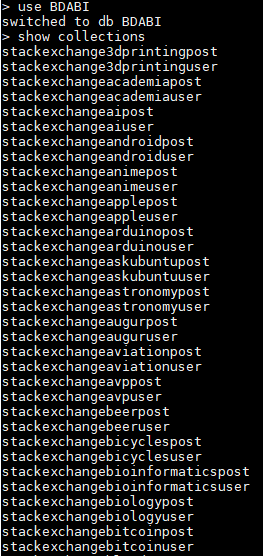
\includegraphics[scale=0.9]{image/mongo1.PNG}
	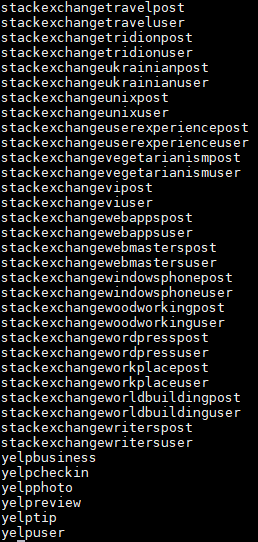
\includegraphics[scale=0.9]{image/mongo2.PNG}
	\caption{MongoDB}
	\label{fig:mongo}
\end{figure}

Conclusasi questa fase, non resta che sfruttare i dati che si dispone per effettuare la ricerca degli esperti su di un determinato argomento. Ricerchiamo gli esperti di \emph{Golf}. Lanciamo il comando in \textbf{Figura \ref{lst:dm}} con golf come topic. Osserviamo un tempo di elaborazione di poco più di 12 minuti. Essa ha coinvolto principalmente il dataset di Yelp, grazie alle recensioni sui campi da golf. Si ottengono gli esperti relativi.

\begin{figure}[H]
	\centering
	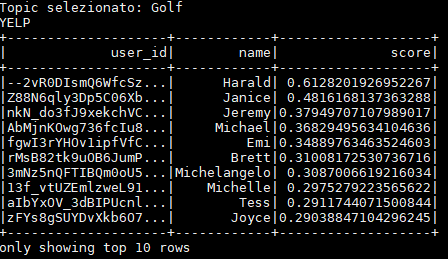
\includegraphics{image/golf.PNG}
	\caption{Esperti di golf}
	\label{fig:golf}
\end{figure}

Analogamente effettuiamo un'ulteriore ricerca di esperti di animali. Osserviamo che il tempo di esecuzione è poco più di 12 minuti. La ricerca è stata effettuata su entrambi i dataset. Risulta interessante osservare le descrizioni che hanno dato gli utenti di loro stessi. La maggior parte di esse fanno riferimento ad un aspetto della vita dell'utente correlato agli animali. Sono dunque persone che reputano il loro rapporto con gli animali come una delle cose primarie da inserire in una descrizione personale.

\begin{description}
\item[Zaralynda]Avid reader, feminist, owned by cats, sometime gamer, and quilter.
Currently share my home with 3 cats.
\item[Yvette Colomb]Animal lover and animal rights activist.
\item[Trond Hansen]I am 53 years old (young). My interests are very broad: science, astronomy, biology, geology, marine biology. I simply want to know how every thing works, I have a cat named Trine. I have always had a cat.
\item[Rebecca RVT]Graduated as Veterinary Technician in spring 2013, got certified in summer of 2013. Currently work primarily with  animal (cats and dogs). I have 11 years experience with exotic pets (pocket pets, reptiles and birds) with 2 years of working at an exotic pet practice.
\item[James Jenkins]I volunteer with \url{http://www.petfinder.com/shelters/PA323.html} Rabbit Wranglers. I can often be found at local community events walking a rabbit on a leash, providing education and offering tips for adopting and rating a pet house rabbit into the family.

\end{description}

\begin{figure}[H]
	\centering
	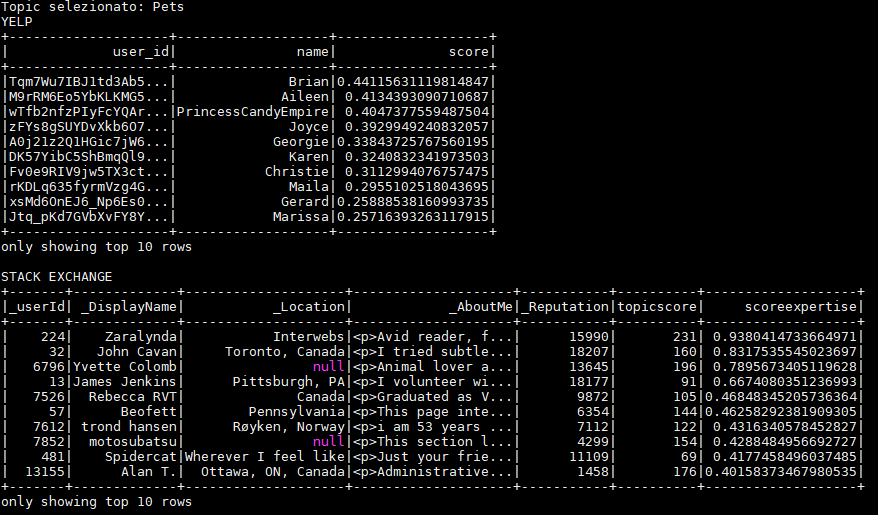
\includegraphics[scale=0.7]{image/pets.PNG}
	\caption{Esperti di animali}
	\label{fig:pets}
\end{figure}
\begin{figure}[H]
	\centering
	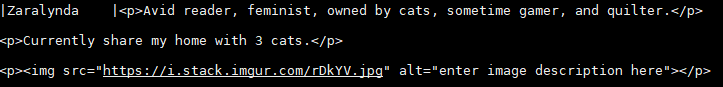
\includegraphics[scale=0.8]{image/pets2.PNG}
	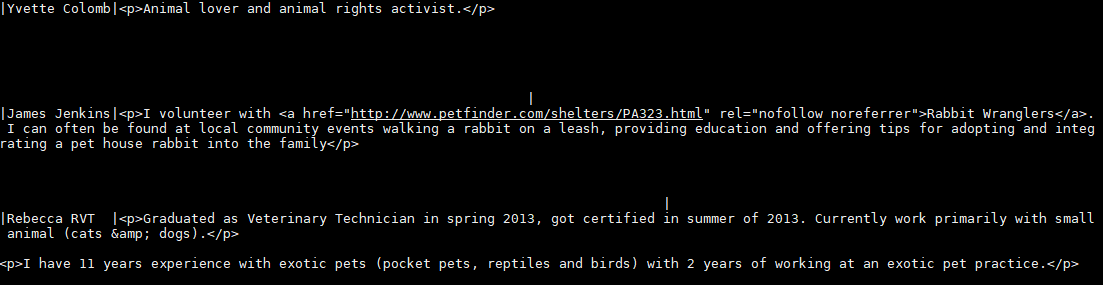
\includegraphics[width=16cm]{image/pets3.PNG}
	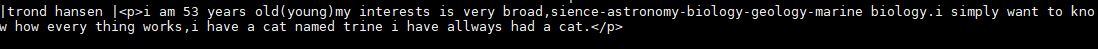
\includegraphics[width=16cm]{image/pets4.PNG}
	\caption{About Me degli esperti di animali}
	\label{fig:abme}
\end{figure}

Al fine di valutare l'algoritmo anche per il dataset Yelp, è stato realizzato un sondaggio con le migliori recensioni ed è stato chiesto ai partecipanti di ordinare gli utenti relativi in base all'esperienza che dimostrano sugli animali. Il sondaggio è stato effettuato su un gruppo ristretto di persone fidate con conoscenza dell'argomento in questione, in modo da garantire la serietà e l'attendibilità del responso. Il ranking ottenuto ricalca quello prodotto dall'algoritmo, eccetto per la quinta posizione. \emph{Georgie}, infatti, è stato posto in fondo alla classifica. Normalmente, con l'argomento \emph{animali}, si sottointende la cura per gli animali. Tutte le recensioni fanno riferimento ad associazioni di volontariato per il salvataggio degli animali, veterinari, attività con degli animali. Georgie, invece, parla di un'attività di ristorazione, che avrà ed accudirà i suoi animali, ma che non farà di ciò il principale business. L'attività è stata dunque classificata in tal modo dal dataset e ben valutata dall'algoritmo per l'ottima recensione ottenuta. Di contro, è stata mal valutata dai partecipanti al sondaggio, abituati dalle altre recensioni a ricercare un altro tipo di competenza nell'utente, più improntata ai temi animalisti. Una parola può rappresentare differenti concetti e a questo punto il tema scivolerebbe sul vero significato dell'argomento animali. Volendoci porre nel punto di vista dell'utilizzatore umano, per il quale è comune essere ambiguo e non specificare pienamente il contesto, sembra comunque accettabile il risultato ottenuto, composto di un unico falso positivo.

\begin{figure}[H]
	\centering
	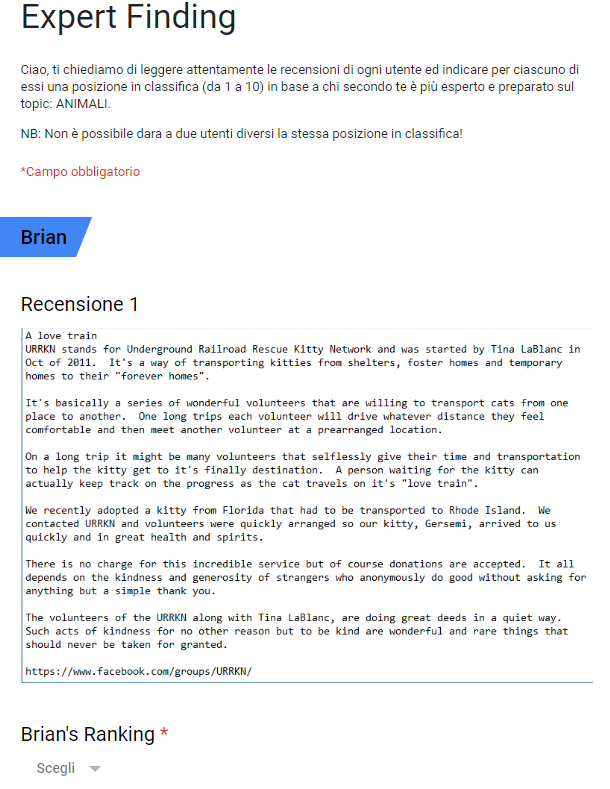
\includegraphics[scale=0.5]{image/form.PNG}
	\caption{Sondaggio sugli esperti di animali}
	\label{fig:frm}
\end{figure}

\begin{figure}[H]
	\centering
	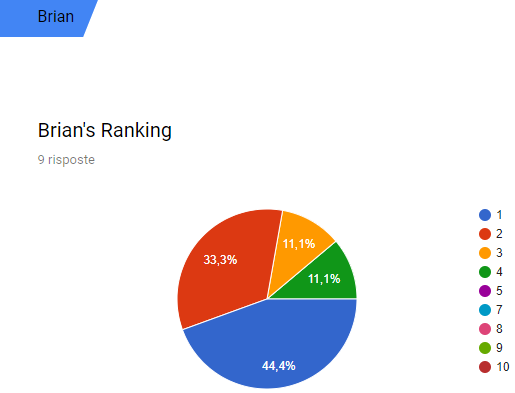
\includegraphics[scale=0.7]{image/sond.PNG}
	\caption{Risultato sondaggio}
	\label{fig:snd}
\end{figure}

Infine ricerchiamo gli esperti di informatica. L'esecuzione impiega 30 secondi e coinvolge solo il dataset di StackExchange. Osserviamo ancora una volta come le descrizioni degli utenti siano coerenti con la tipologia di esperto cercata: un ricercatore del Technion, un ingegnere del software di Google, un dottorando dell'Università di British Columbia, un professore dell'Università dell'Illinois.

\begin{description}
\item[Yuval Filmus]Assistant Professor in the Department of Computer Science at the Technion.
\item[Raphael]I am a computer scientist by training, which means I now think like one: always analysing,  abstracting, reducing, problem solving. In addition, I picked up some affection and, hopefully, ability for actually building software over the years. You can take a look over on \url{https://github.com/reitzig} Github. During my time at university I have found a passion for teaching, by which I mean helping people learn. Some say I was quite the nitpicker; it's for your best, I promise! In my free time I play games, read books, code, work out, enjoy music, and roam the webs.
\item[Kaveh]\url{http://ca.linkedin.com/in/ghasemloo} Software Engineer at \url{http://www.google.com} Google. Ph.D. in Computer Science, \url{https://www.utoronto.ca/} University of Toronto, \url{http://web.cs.toronto.edu/} Department of Computer Science, \url{http://www.cs.toronto.edu/theory/index.php} Theory Group. Thesis: \url{http://www.cs.toronto.edu/~kaveh/papers/phd-thesis.pdf} "Uniformity and Nonuniformity in Proof Complexity", 2016. Ex-moderator on \url{http://cstheory.stackexchange.com} cstheory.
\item[Jmite]I am Joey Eremondi, a PhD Student at the \url{https://www.cs.ubc.ca/} University of British Columbia. I do research in Programming Languages and Theory of Computation, particularly with dependent types. My \url{http://dspace.library.uu.nl/handle/1874/337692} Masters Thesis was on improving error messages for higher order unification. I've also co-authored a few papers on reversal-bounded counter automata. I have an M.Sc in Computing Science from \url{http://www.cs.uu.nl/} Utrecht University, a B.Sc. Honours in Computer Science, and a B.Sc. 4-year in Mathematics, both from the \url{http://www.usask.ca/" rel=} University of Saskatchewan.
\item[JeffE]I am a full professor of \url{http://www.cs.uiuc.edu} computer science at the University of Illinois, Urbana-Champaign.  I teach \url{http://www.cs.uiuc.edu/~jeffe/teaching/algorithms} algorithms.

\end{description}

\begin{figure}[H]
	\centering
	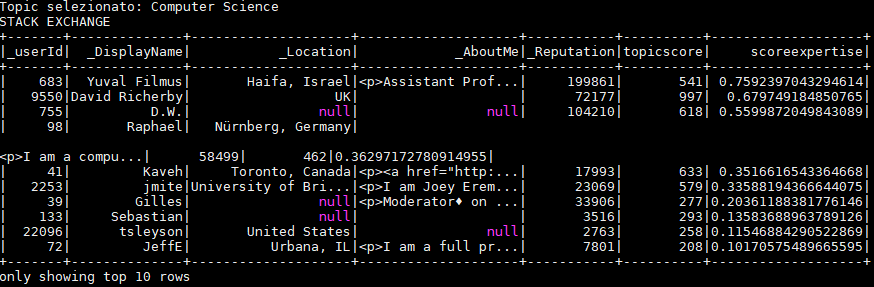
\includegraphics[scale=0.7]{image/cs.PNG}
	\caption{Esperti di informatica}
	\label{fig:cs}
\end{figure}

\section{Tempi e costi}
La metrica di valutazione della competenza riesce efficacemente ad individuare gli esperti nel settore. I tempi di esecuzione sono confermati anche con prove ripetute e con differenti topic. Le differenze sostanziali nei tempi di elaborazione sono dovute alla composizione dei dataset. Essendo StackExchange già suddiviso per topic, presenterà un numero di tuple nettamente inferiore alle centinaia di migliaia di Yelp, che mantiene i dati di tutta la piattaforma senza scrematura. La composizione di Yelp necessita inoltre di un'operazione di Join aggiuntiva per ricavare i topic dalle aziende, e di conseguenza le recensioni relative. Una fase di preprocessing onerosa potrebbe catalogare i dati di Yelp per topic nel database, riducendo i tempi di esecuzione ma provocando più ridondanza e maggior consumo di memoria. Questa è una strada al momento non praticabile per le poche risorse di memoria a disposizione nella macchina virtuale. Differenti configurazioni tecniche di Spark, variando il numero di esecutori, di core per ciascuno di essi, e di memoria loro disponibile, possono portare ad una riduzione dei tempi globali di al più 10 secondi, suggerendo che non siano le limitazioni tecniche della piattaforma a vincolare eccesivamente i tempi. Per quanto riguarda i costi in termini di risorse di memoria utilizzate, il disco primario non è stato sufficiente per l'estrazione e la memorizzazione dei dati. Si è quindi ricorso al disco temporaneo maggiormente capiente ma volatile. Sono quindi stati trovati dei compromessi tra tempi e costi per far fronte alla esigua disponibilità di risorse di memoria. La memoria centrale per l'elaborazione, invece, si è dimostrata sufficiente per garantire un'esecuzione efficiente.